\documentclass[conference]{IEEEtran}
\IEEEoverridecommandlockouts%

% Packages
\usepackage{cite}
\usepackage{amsmath,amsfonts}
\usepackage{algorithm}
\usepackage{algpseudocode}
\usepackage{graphicx}
\usepackage{textcomp}
\usepackage{xcolor}
\usepackage{booktabs}
\usepackage{adjustbox}
\usepackage{listings}
\usepackage{bm}
\usepackage{hyperref}
\usepackage{cleveref}
\usepackage{svg}

\usepackage{pgfplots}
\pgfplotsset{compat=newest}
\usepackage{siunitx}

\usepackage{verbatim}
\usepackage{multirow}

\graphicspath{{./img/}}

\def\BibTeX{{\rm B\kern-.05em{\sc i\kern-.025em b}\kern-.08em
    T\kern-.1667em\lower.7ex\hbox{E}\kern-.125emX}}

\begin{document}

\title{Deliverable report \\
\footnotesize \textit{``Alessio Blascovich'': Mat: 257561, \texttt{alessio.blascovich@studenti.unitn.it}, GitRepo: \texttt{https://github.com/elblasco/GPU-Computing-2025-257561}}}

\maketitle

\begin{abstract}
%[max 200 words]\\
The sparse matrix-dense vector multiplication (SpMV) is an algebraic operation in which a sparse matrix is multiplied by a dense vector. SpMV is widely used in real-world applications such as scientific and engineering computing, data mining, and graph analysis.

This deliverable discusses the implementation and the performance analysis of a series of SpMV algorithms for COO matrices. These algorithms are implemented for a single-core CPU and a \emph{CUDA} capable GPU. Regarding the GPU implementations, no threads/warp level synchronisation has been used, only atomic operations to keep the resulting vector consistent.
\end{abstract}

\begin{IEEEkeywords}
Sparse Matrix, SpMV, \emph{CUDA}, Parallelization, Storage Format
\end{IEEEkeywords}

\section{Introduction}
SpMV is considered a fundamental algebraic operation in many scientific fields such as computational fluid dynamics, optimisation and graph algorithms.

The main challenges in implementing an efficient SpMV algorithm differ in CPU and GPU, and are strictly bound to the type of matrix representation used (COO, CSR, ELL,\dots). For the purpose of this deliverable only COO representation is taken into account.

From the CPU point of view, the main issue is to maximise the cache hits throughout the execution, data consistency is not a problem since only single core CPUs were used.

On the GPU side the problem of maximising cache hits remains, and on top of that, race conditions are added. Since in COO format the length of a row is not specified, multiple threads could be reading different portions of the same row and therefore, writing on the same output memory area.

\section{Problem Statement}
The SpMV operation is formally defined in~\Cref{eq:1}, where \(\bm{A}\) is a \(n\times m\) sparse matrix, \(\bm{X}\) a \(m\times 1\) dense vector and \(\bm{Y}\) another \(n\times 1\) dense vector.

\begin{equation}\label{eq:1}
\bm{Y} = \bm{A}\cdot\bm{X}
\end{equation}

\subsection{Storage Format}
The COOrdinate format (COO) is a representation for sparse matrices. COO uses 3 different arrays to store al the necessary information. One array is dedicated to store all the values, while the other 2 contain the corresponding row and column indices, ideally the arrays are sorted first by row index and then by columns index. An example of a COO encoding is shown in~\Cref{fig:coo-format}.

\begin{figure}[ht]
  \centering
  % \includesvg[width=\columnwidth, height=30ex]{COO-format.svg}
  \includesvg[width=\columnwidth]{COO-format.svg}
\caption{encoding of a matrix on COO format}\label{fig:coo-format}
\end{figure} 

\subsection{Parallelization}\label{sec:parallelization}
Three different kernels have been used for the \emph{CUDA} capable GPU. Although they differ by the kind of memory and optimisations used, all of them leverage on the fact that the COO arrays are sorted first by row  and then by column. In general the multiplication problem has been reduced to a prefix sum computation. In to optimise the computation of prefix I tried to minimise global memory writes by using warp level primitives and the shared memory.

\section{State of the Art}
%Describe the available library solutions for the SpMV problem, including references and citations \cite{asimov1950irobot, svevo1923coscienza, pirandello1926uno}.
Starting from the implementations presented in this deliverable, performances could be drastically enhanced. Fukaya et al.~\cite{fukaya2021}, despite focussing on the HDC storage format, improved the SpMV CPU based by exploiting diagonalization patterns, SIMD instructions and \emph{OpenMP} directives. On the GPU side Chu et al.~\cite{chu2023} used the CSR format and a more sophisticated load balancing to improve the performances. NVIDIA itself made available a set of libraries to manage and use COO formatted matrices, namely \emph{cuSPARSE}.

In the NVIDIA library \emph{cuSPARSE}, and many others commercial libraries, the problem is redefined according to~\Cref{eq:2}.

\begin{equation}\label{eq:2}
\bm{Y} = \alpha\emph{op}(\bm{A})\cdot\bm{X}+\beta\bm{Y}
\end{equation}

With \(\alpha\) and \(\beta\) being two scalars, and \emph{op} being a matrix transformation such as a transposition.
\section{Methodology and Contributions}\label{sec:methodology}
% Describe the methodology used during the analysis, the compared algorithms and the expected outcomes. Use pseudo-codes like Algorithm \ref{alg:COOaggr} to describe your own implemented kernels.

The test were carried out on a remote cluster. I compared all the kernels against a set of matrices, for every kernel I executed multiple run to collect more meaningful data.

All the algorithms assumed that the resulting array is empty, so I explicitly initialised every element of it to the value 0.

\subsection{Algorithms}

For the GPU implementation I have developed three kernels, they are divided into two main categories. Kernel that leverage on shared memory and kernels that leverage on warp level primitives. \Cref{alg:warp} was the first kernel developed using warp-level primitives. Every thread proceed with a striding of \(\mathit{numThreads}\) values, initially every thread computes the product between its the matrix value and the value for the corresponding dense array. This values are then combined using a prefix-sum based on warp-level instructions.

\begin{algorithm}[ht]
\caption{SpMV algorithm with WARP level primitives}
\algorithmicrequire~The input vectors \(val\), \(row\) and \(col\) of size \(nnz\), array \(arr\) of size \(columns\) and an array \(res\) of size \(rows\).
\begin{algorithmic}[1]\label{alg:warp}
\Procedure{Function}{\(row\), \(col\), \(val\), \(arr\), \(res\), \dots}
  \State\(start\gets threadId\)
  \State\(pos\gets threadId\&(WARP\_SIZE - 1)\)
  \State\(total\gets gridDim\cdot blockDim\)
  \For{\(i\) in \(\{start\dots nnz\}\) with \(i = i + total\)}
    \State\(row\_id\gets row[i]\)
    \State\(col\_id\gets col[i]\)
    \State\(val\_id\gets val[i]\)
    \State\(//The\ last\ thread\ per\ row\ writes\)
    \State\(row\_next\gets shfl\_down(\texttt{0xff}\dots, row, 1)\)
    \If{\ensuremath{\mathit{Edge\_detection()}}}
      \State\texttt{atomicAdd(\&res[row], prod)};
    \EndIf%
  \EndFor%
\EndProcedure%
\end{algorithmic}
\end{algorithm}

\begin{algorithm}[ht]
\caption{Prefix-sum with WARP level primitives}
\algorithmicrequire~The values for \(product\), \(row\) and \(pos\).
\begin{algorithmic}[1]\label{alg:sum-warp}
  \Procedure{prefix\_sum\_warp}{\ensuremath{product, row, pos}}
    \For{\(x\) in \(\{1\dots WARP\_SIZE\}\) with \(x = x\cdot 2\)}
      \State\(prev\_row\gets shfl\_up(\dots, row, x)\)
      \State\(prev\_prod\gets shfl\_up(\dots, product, x)\)
      \If{\(pos\geq delta\land prev\_row = row\)}
        \State\(product = product + rev\_prod\)
      \EndIf%
    \EndFor%
  \EndProcedure%
\end{algorithmic}
\end{algorithm}

\begin{figure}[ht]
  \centering
  \includesvg[width=\columnwidth]{warp-level.svg}
\caption{Execution of prefix sum with warp size 8}\label{fig:warp-sum}
\end{figure}

As mention in~\Cref{sec:parallelization} I reduced the problem to a prefix sum, as a matter of fact~\Cref{alg:sum-warp} exploits warp-level primitives to compute a prefix sum. \Cref{alg:sum-warp} is more refined w.r.t. simple prefix sum, since it has to take into account the possibility that within the same warp we could be summing different rows. In~\Cref{fig:warp-sum} it is described a possible execution for the prefix sum procedure, in red the value returned summed in global memory in line 12 of~\Cref{alg:warp}. The next improvement introduced was the loop unroll of the main loop in~\Cref{alg:sum-warp}, using compiler directives. To be precise, I used \texttt{\#pragma unroll}, since the loop always iterates in an interval known at compile time, in fact \texttt{WARP\_SIZE} is a macro defined as the value 32.

I also tried to improve the baseline proposed in deliverable 1 by using dynamically allocated shared memory.


% From the theory Algorithm~\ref{alg:striding} should have been faster. This follows from the fact that every thread within the same SM (Streaming Multiprocessor) accesses elements that are spacially adjacent in the memory. Contrary, Algorithm~\ref{alg:contiguous} has an higher rate of cache miss since, threads in the same SM may need to access elements far away from each other. Since the cache optimisation is so important for these algorithm and they had to do so few floating point operations I expected for them to be memory bounded.

\section{System Description and Experimental Set-up}

%Use this section to describe system, dataset and experimental set-up.

\subsection{System Description}

%Describe the used system and the software environment (CUDA version, GCC version, \dots). Decide which information are valuable to group into a table like Table \ref{tab:system_description} and which are more valuable to be described in the text.

For this deliverable I could not use my own machine since it does not have a \emph{CUDA} capable GPU, so I only used the remote cluster. \Cref{tab:system-softwares} describes all the software used, while~\Cref{tab:system-detals} describe the hardware that I used.

\begin{table}[ht]
    \centering
    \begin{tabular}{llll}
      \toprule
      \textbf{Software} & \textbf{Version} & \textbf{Git Branch} & \textbf{Git Hash}\\
      \midrule
      \texttt{GCC} & 11.5.0 & & \\
      \texttt{CUDA} & 12.5.0 & & \\
      \texttt{SbatchMan} & & example & 40d869a\\
      \texttt{distributed\_mmio} & & main & 3563a2f\\
      \bottomrule
    \end{tabular}
    \vspace{.5em}
    
    \caption{Systems softwares}
    \label{tab:system-softwares}
\end{table}

\begin{table}[ht]
    \centering
    \begin{adjustbox}{width=\columnwidth}
    \begin{tabular}{llrl}
    \toprule
    \textbf{Processor} & \textbf{Cores per Socket} & \textbf{RAM} & \textbf{Accelerator} \\
    \midrule
    Intel(R) Xeon(R) Silver 4214 & 48 at 2.2 GHz & 400 GB & NVidia L40s\\
    \bottomrule
    \end{tabular}
    \end{adjustbox}
    \vspace{.5em}
    
    \caption{Systems details}
    \label{tab:system-detals}
\end{table}

\subsection{Dataset description}

%Discribe the used dataset and the reasons of your choice. List the used input matrices and all the information that you think are valuable to show (number of non-zero elements, sparsity ratio, \dots); Table \ref{tab:my_label} gives you a possible example.

To add a bit more of generality to the dataset I picked six matrix from six different kinds from the site \url{https://sparse.tamu.edu/}. Since all the matrices are squared only the number is written on~\Cref{tab:dataset}.

\begin{enumerate}
\item Electromagnetics Problem;
\item Undirected Weighted Graph;
\item Optimization Problem;
\item Structural Problem;
\item 2D/3D Problem;
\item Semiconductor Process Problem.
\end{enumerate}

\begin{table}[ht]
    \centering
    \begin{tabular}{lrrr}
    \toprule
    \textbf{Name} & \textbf{Rows} & \textbf{Pattern Entries} & \textbf{Sparsity Rate}\\
    \midrule
      \texttt{dielFilterV3real} & 1,102,824 & 89,306,020 & \(7\mathrm{e}{-5}\)\\
      \texttt{Flan\_1565} & 1,564,794  & 117,406,044 & \(5\mathrm{e}{-5}\)\\
      \texttt{Flan\_1565} & 1,564,794  & 117,406,044 & \(5\mathrm{e}{-5}\)\\
      \texttt{mawi\_201512020330} & 226,196,185 & 480,047,894 & \(9\mathrm{e}{-9}\)\\
      \texttt{nlpkkt160} & 8,345,600 & 229,518,112 & \(3\mathrm{e}{-6}\)\\
      \texttt{vas\_stokes\_2M} & 2,146,677 & 65,129,037 & \(1\mathrm{e}{-5}\)\\
      \bottomrule
    \end{tabular}
    \vspace{.5em}
    \caption{Input Matrices}
    \label{tab:dataset}
\end{table}

\subsection{Experimental Set-up}
% Explain the benchmark metrics and all the experimental set-up (warm-up cycles, number of performed runs\dots).

For every matrix I measured a set of metrics using an approach similar to the first deliverable. For every matrix I spawned a job which ran multiple times every kernel and gathered info about the performances. The metrics measured were: execution time, peak GFLOP/s developed and peak bandwidth used. I was able to test all the algorithms in a single job since I switched to the node \emph{edu02}, which is equipped with the more powerful NVidia L40s, w.r.t. \emph{edu01} which is equipped with NVidia A30.

Every job carried out its measurements performing multiple runs of the same kernel. The kernel tests were split into two period, a warm-up period and a ``valid'' period, the data has been collected only during the ``valid'' period. The distinction were necessary in order to war-up the GPU caches.

To automatise the matrix parsing, and their conversion in binary format, I used a fork of \texttt{distributed\_mmio}\footnote{The fork author is Matteo Di Noia \url{https://github.com/matteo-dinoia/distributed_mmio} while I just fixed some minor issues \url{https://github.com/elblasco/distributed_mmio}}.

The job submission were managed by \emph{SbatchMan}, this automation allowed me to create multiple experiments and submit all of them. In  particular I created an experiment for normal metrics gathering and an experiment for profiling via \emph{nsys}, \emph{ncu} and \emph{nvtx}.

\section{Experimental Results}\label{sec:result}
% Present and discuss results. Include plots and tables when required (like Figure \ref{fig:enter-label}). Do not simply describe the figures; criticise the achieved results by underlining how they confirm/differ from the expected outcomes described in Section \ref{sec:methodology}.
\begin{figure}[ht]
    \centering
    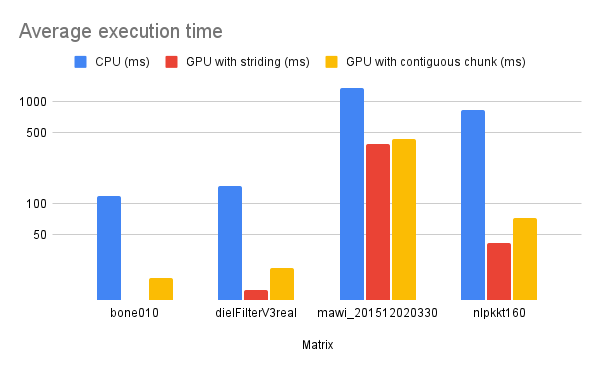
\includegraphics[width=0.95\linewidth]{average-execution-time.png}
    \caption{Average Execution Time (lower is better)}
    \label{fig:avg-exec-time}
\end{figure}

\begin{figure}[ht]
    \centering
    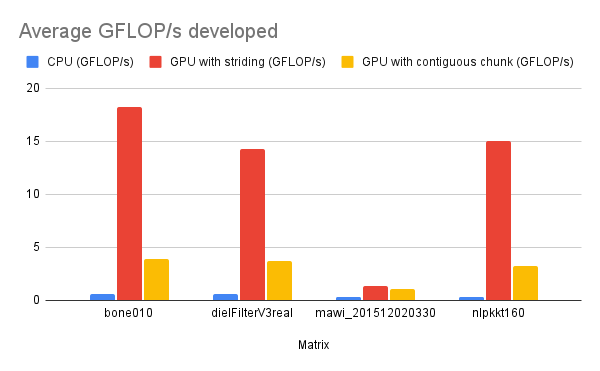
\includegraphics[width=0.95\linewidth]{average-gflop.png}
    \caption{Average GFLOP/s Developed (lower is better)}
    \label{fig:avg-gflop}
\end{figure}
As expected in~\Cref{sec:methodology} and shown in~\Cref{fig:avg-exec-time, fig:avg-gflop},~\Cref{alg:striding} is faster than all the other implementations.
\begin{figure}[ht]
    \centering
    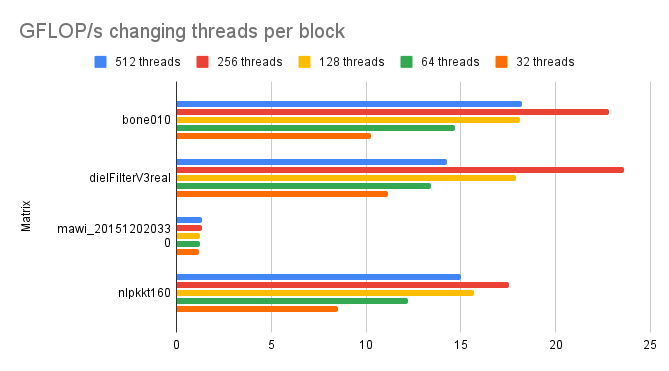
\includegraphics[width=0.95\linewidth]{gflop-block.png}
    \caption{GFLOP Compared The Number Of Threads Per Block}
    \label{fig:gflop-block}
\end{figure}

\begin{figure}[ht]
    \centering
    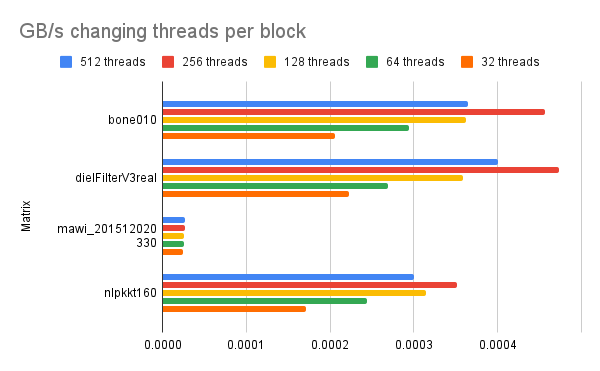
\includegraphics[width=0.95\linewidth]{gb-block.png}
    \caption{GB/s Compared The Number Of Threads Per Block}
    \label{fig:gb-block}
\end{figure}
I decided to dig a bit more into the performances of~\Cref{alg:striding} by changing the maximum amount of thread per block. Starting from the base of 512 threads I divided by 2 until reaching 32, i.e., the size of warp. The optimal amount of threads per block resulted to be 256. This is due to the use of an atomic instruction within the code, the semantic of the instruction make concurrent write over the same address sequential; in this case if two threads are working on the same row their sum operations will sequentialised since they are trying to write on the same result address. Using less threads,.i.e., each thread works on more elements; conflicts (threads working) on the same row are reduced to a minimum. However, this minimum is not stable, in fact decreasing again the value to 128, 64 or 32 the performances decreases again, this could be symptom of either:
\begin{itemize}
\item too few threads working, so an excessive workload for each of them;
\item too much threads working on the same row, hence an high number of conflicts on the same row.
\end{itemize}
Unfortunately, I was not able to determine a more fine grain optimisation, since the optimal size depends on the input matrix shape. \Cref{fig:gflop-block, fig:gb-block} highlights the fact that the variations of performances are not constant over all the matrices considered.

\begin{figure}[ht]
\centering
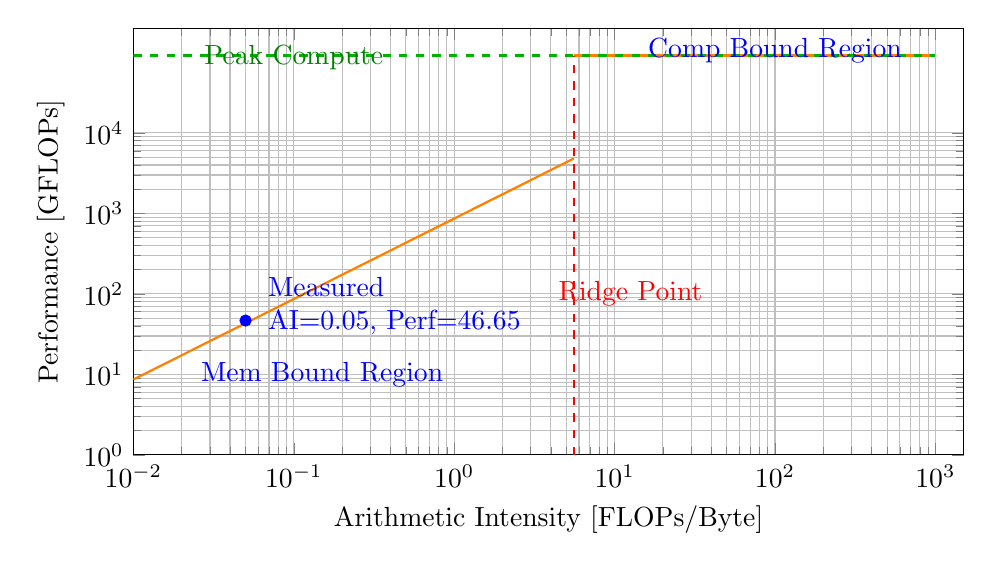
\begin{tikzpicture}
\begin{loglogaxis}[
    width=\linewidth,
    height=7cm,
    xlabel={Arithmetic Intensity [FLOPs/Byte]},
    ylabel={Performance [GFLOPs]},
    %title={Roofline Model for NVIDIA L40s GPU (FP32)},
    grid=both,
    xmin=0.01, xmax=1500,
    ymin=1, ymax=200000,
    xtick={0.01, 0.1, 1, 10, 100, 1000},
    ytick={1, 10, 100, 1000, 10000}
]


% --- Parameters ---
\def\ridgepoint{5.57}     % FLOPs/Byte
\def\peakcompute{91600}    % GFLOPs
\def\bandwidth{864}       % GB/s
\def\ArithmeticIntensity{0.05}
\def\performance{46.65}

% --- Roofline: Memory-bound and compute-bound ---
\addplot[
    domain=0.01:\ridgepoint,
    samples=200,
    thick,
    orange
] {\bandwidth * x}; % Memory-bound line

\addplot[
    domain=\ridgepoint:1000,
    samples=2,
    thick,
    orange
] {\peakcompute}; % Compute-bound line

% --- Dashed Ridge point ---
\addplot[dashed, red, thick] coordinates {(\ridgepoint, 1) (\ridgepoint, \peakcompute)};
\node[red] at (axis cs:\ridgepoint + 7, 100) {Ridge Point};

% --- Measured point ---
\addplot[
    only marks,
    mark=*,
    mark size=2pt,
    color=blue
] coordinates {(\ArithmeticIntensity, \performance)};
\node[align=left, anchor=west, blue] at (axis cs:0.06, 70) {Measured\\AI=0.05, Perf=46.65};

% --- Peak compute line (green dashed) ---
\addplot[dashed, green!70!black, thick] coordinates {(0.01, \peakcompute) (1000, \peakcompute)};
\node[anchor=south, green!50!black] at (axis cs:0.1, \peakcompute/2) {Peak Compute};

% --- Annotations ---
\node[blue] at (axis cs:0.15, 10) {Mem Bound Region};
\node[blue] at (axis cs:100, \peakcompute + 15000) {Comp Bound Region};

\end{loglogaxis}
\end{tikzpicture}
\caption{Roofline Model For SpMV On NVIDIA L40s}
\label{fig:roofline}
\end{figure}

Following the NVIDIA's white-paper for the A30, I drew the roofline model for single precision floating point, since in my code I used \texttt{float} as data type to represent values within the matrix and vectors. \Cref{fig:roofline} highlights the fact that my \emph{CUDA} kernels are indeed a memory bounded.

\section{Conclusions}
The presented algorithms are far from decent implementations. The representation used for the matrices is sub-optimal since the length of a row is unknown a priori, therefore it is impossible to do a decent load balancing between the threads. For better GPU performances using another representation such as CSR would works better.

Another bottleneck for the algorithm is represented by the use of an atomic instruction. Instead of this instruction thread/warp level synchronisation should be used.

On the CPU side, this representation is optimal since it permits to maximise the number of cache hits working on data stored so closely.

\bibliographystyle{IEEEtran}
\bibliography{references}

\end{document}

